\documentclass[times, utf8, diplomski]{fer}
\usepackage{booktabs}
\usepackage{float}
\usepackage{subcaption}

\newcommand{\source}[1]{\vspace{-12pt} \caption*{\textbf{Source}: {#1}} }
\renewcommand{\labelitemi}{\textbullet}

\begin{document}

% TODO: Navedite broj rada.
\thesisnumber{000}

% TODO: Navedite naslov rada.
\title{Naslov}

% TODO: Navedite vaše ime i prezime.
\author{Arthur Dent}

\maketitle

% Ispis stranice s napomenom o umetanju izvornika rada. Uklonite naredbu \izvornik ako želite izbaciti tu stranicu.
\izvornik

% Dodavanje zahvale ili prazne stranice. Ako ne želite dodati zahvalu, naredbu ostavite radi prazne stranice.
\zahvala{}

\tableofcontents

\chapter{Uvod}
Kada se govori o biologiji i medicini, dvije grane koje se bave proučavanjem života i načina funkcioniranja živih bića, svi se slažu da su izuzetno puno napredovale sa razvojem tehnologije. Ljudi razvijaju sve složenije i sve preciznije alate, strojeve i programe za proučavanje svih sustava u tijelu, od stanice do skupa organa koji rade zajedno, kao jedan, te skupa čine savršeno ugođeni sustav. No u jednom području tih znanosti ne napreduje se tom brzinom kao u ostalim područjima. O tom području i sustavu organa nezna niti približno mnogo kao o ostalim organima i sustavima u tijelu. Znanstvenici govore da je to najsloženiji sustav, najjače super-računalo na svijetu. Centar tog sustava je mozak, organ koji može probaviti nevjerojatnu količinu informacija u stvarnom vremenu sa gotovo savršenom preciznosti. \par

Od početka "modernog doba čovječanstva", javlja se ideja umjetne inteligencije. Znanstvenici iz područja tehničkih znanosti i računarstva teže razvijanju nečeg takvog i prirodno se nameće ljudski mozak kao ideal, razina inteligencije koju se želi dostići. Pretpostavlja se da je najveći dio mozga, oko 2/3, posvećen vidu \citep{vision_percentage}. Iz tog razloga, veliki dio proučavanja i razvoja moderne umjetne inteligencije fokusirano je na vid. U nastavku rada dan je pregled najvažnijih algoritama i arhitektura mreža.

\chapter{Računalni vid}
\section{Računalni vid}
Računalni vid je veliko područje računarske znanosti koje se bavi algoritmima i metodama vezanim za obradu slike. Kao što je navedeno u uvodu, vid je osjetilo preko kojega ljudi primaju najviše informacija, više nego preko bilo kojeg drugog osjetila. Da bi bilo moguće napraviti stroj ili program koji vidi kao mi, prvo je potrebno shvatiti kako ljudi vide i kako obrađuju informacije primljene preko očiju. Samo shvaćanje kako funkcionira ljudski vid je izuzetno težak zadatak. Danas donekle razumijemo taj proces, no ima još puno stvari koje su ostale neodgovorene. Recimo, istraživanja pokazuju da ljudi mogu prepoznati što je na slici za samo 13 milisekundi\citep{RSVP13ms}. Ljudi i dalje ne znaju kako mozak to radi. Postoje nagađanja, no ništa nije dokazano i upitno je hoće li ikada ti koncepti biti do kraja shvaćeni i objašnjeni. Zbog složenosti ovog problema, nemoguće je naći riješenje klasičnim pristupom i napisati program eksplicitno. Zato se u ovakvim problemima pribjegava umjetnoj inteligenciji.
Postoji nekoliko dijelova cijelog sustava vida koji ljudima omogućavaju vid:
\begin{itemize}
\item{\textbf{Vidjeti}} - dati računalu vid znači dati mu oči. U tom području znanost je dosta napredovala tako da danas postoje kamere sa većom rezolucijom od ljudskog oka. Ovaj dio vida odvija se, naravno, u samom oku.
\item{\textbf{Prepoznati}} - moći prepoznati različite objekte, maknuti šum sa slike itd. Ukratko, vidjeti što se na slici nalazi. Ovaj aspekt vida odvija se unutar oka i na putu do mozga gdje mozak na kraju posloži sve te informacije u smislenu sliku.
\item{\textbf{Razumijeti}} - shvatiti što se na slici nalazi, shvatiti odnose među objektima, propoznati različite predmete iz različitih kuteva... Ljudski mozak sposoban je prepoznati jabuku bila ona crvena, žuta ili zelena. Sposoban je prepoznati jabuku i ako je napola pojedena. Sposoban je prepoznati jabuku neovisno o njenoj orjentaciji, neovisno o tome miruje li ili se kreće. Ovaj dio vida odvija se potpuno u mozgu. Ovdje je trenutno dosegnuta granica računalnog vida i umjetne inteligencije. No, to ne znači da je nemoguće ići dalje, nego samo da je znanost savladala dosadašnje probleme i trenutno se bavi ovim dok ne nađe riješenje. 
\end{itemize}

\section{Kategorije računalnog vida}
Računalni vid podjeljen je u nekoliko kategorija:
\begin{enumerate}
\item \textbf{Klasifikacija i Lokalizacija.} Ovo područje računalnog vida bavi se prepoznavanjem objekata na slici. To znači da algoritam odlučuje kojem razredu (\textit{engl.} class) pripada cijela slika. Pretpostavljajući navedeno, lokalizacija je proces pronalaženja pozicije objekta na slici. Rezultat procesa lokalizacije obično je crtanje okvira (\textit{engl.} bounding box) oko objekta na slici. Pobjednici natjecanja "Large Scale Visual Recognition Challenge 2017 (ILSVRC2017)" u kategoriji klasifikacije pobijedili su sa rezultatom od 2.251\% pogreške, dok su pobjednici u kategoriji lokalizacije postigli rezultat sa greškom od 6.226\%. Sa slike \ref{img:ILSVRC} vidi se da su se razultati u odnosu na 2016. godinu popravili za 0.8\% u kategoriji klasifikacije te 1.5\% u kategoriji lokalizacije .
\begin{figure}[htb]
\centering
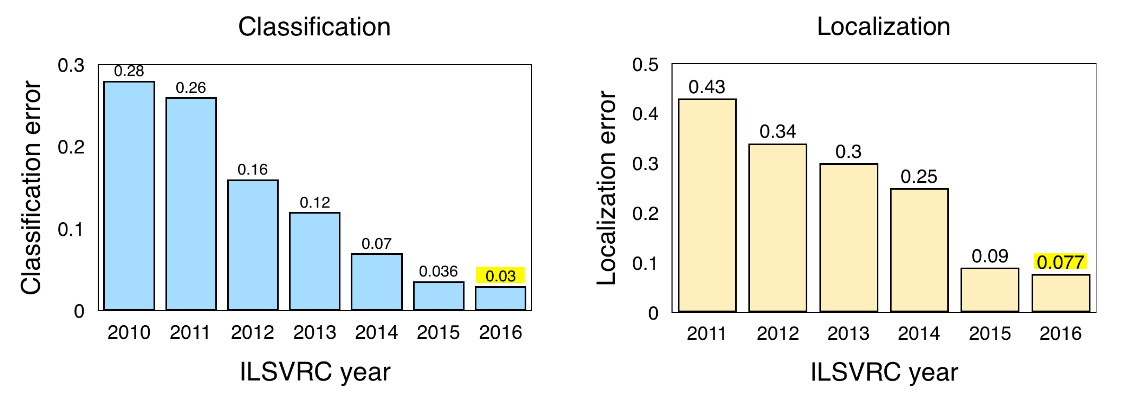
\includegraphics[width=\linewidth]{img/ILSVRC.png}
\caption{Rezultati natjecanja ILSVRC tijekom godina \citep{ILSVRC}}
\label{img:ILSVRC}
\end{figure}

\item \textbf{Detekcija.} Pod pojmom detekcija podrazumijeva se pronalaženje objekata na slici, odnosno, određivanje prisutnosti objekata na slici. Proces detekcije objekata je malo složeniji od kalsifikaije/lokalizacije objekata zbog toga što se ovdje mora provesti više klasifikacija i lokalizacija na jednoj slici te objekti mogu biti iz više domena. Pri klasifikaciji projeravamo pripada li objekt nekom razredu objekata i dobijamo binarni odgovor (\textit{pripada} ili \textit{ne pripada} dani objekt danom razredu), dok je pri detekciji potrebno provesti taj postupak za sve moguće razrede objekata.
\begin{figure}[htb]
\centering
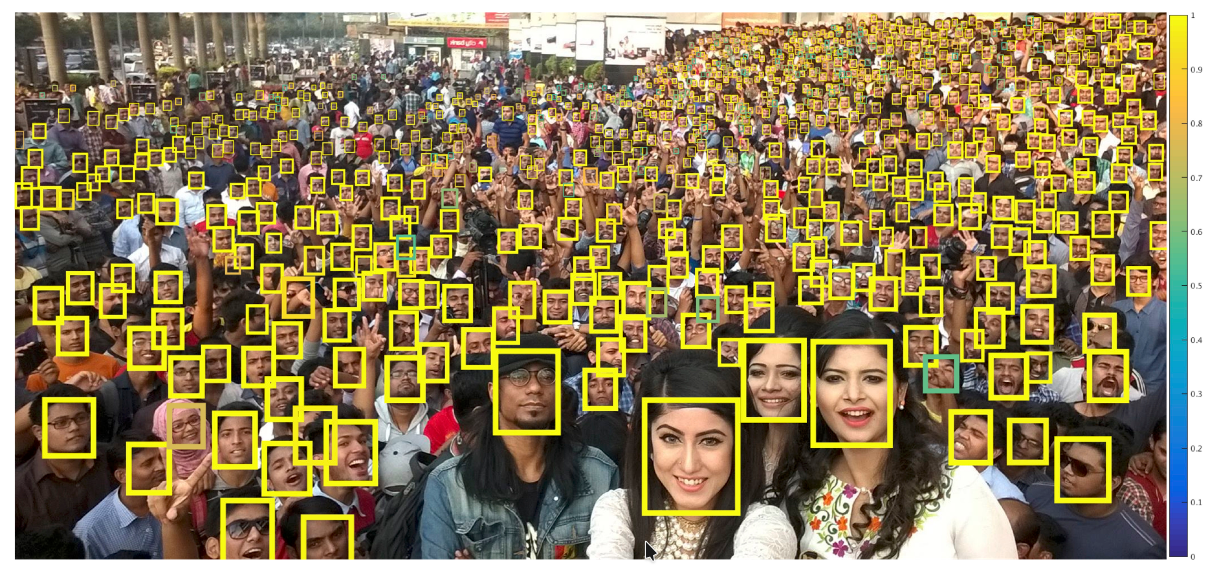
\includegraphics[width=\linewidth]{img/FindingTinyFaces.png}
\caption{Rezultati algoritma za detekciju lica iz rada \citep{TinyFaceDetector}}
\label{img:findingTinyFaces}
\end{figure}

\item \textbf{Praćenje.} Ovaj pojam odnosi se na praćenje određenog objekta ili više njih u sceni. Ova kategorija se, logično, primjenjuje samo u području videa i izuzetno je bitna za sustave koji riješavaju zadatke poput autonomne vožnje.

\item \textbf{Segmentacija.} Pojam segmentacije odnosi se na proces grupiranja piksela u skupine s kojima se kasnije može raditi niz drugih procesa, npr. klasifikacija itd. 

\begin{figure}[htb]
	\centering
	\begin{subfigure}[b]{0.4\linewidth}
		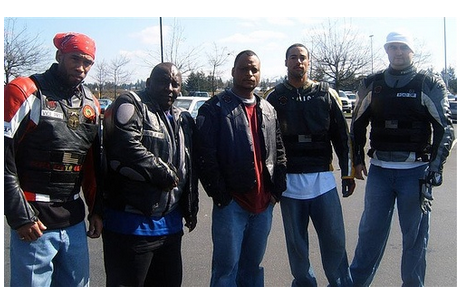
\includegraphics[width=\linewidth]{img/OriginalImage.png}
		\caption{Originalna slika}
	\end{subfigure}
	\begin{subfigure}[b]{0.4\linewidth}
		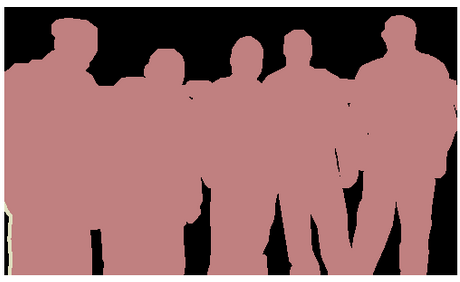
\includegraphics[width=\linewidth]{img/ImageSegmentation.png}
		\caption{Segmentirana slika}
	\end{subfigure}
	\caption{Segmentacija slike (Pascal VOC2007)}
	\label{img:segmentation}
\end{figure}

Nadalje, semantička segmenatacija, kako i samo ime govori, pokušava odrediti semantičku ulogu svakog piksela u slici. Dakle, možemo reći da pokušava klasificirati svaki piksel u njegovu semantičku cjelinu. 

\begin{figure}[htb]
\centering
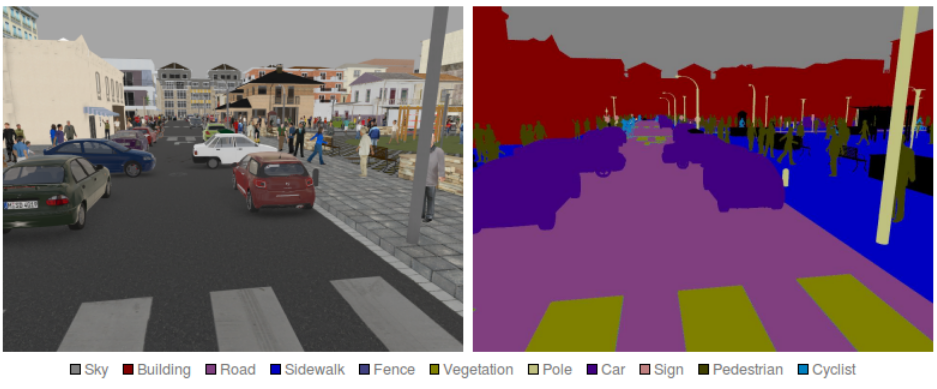
\includegraphics[width=\linewidth]{img/SemanticSegmentation.png}
\caption{Semantička segmentacija slike (SYNTHIA skup podataka)}
\label{img:semanticSegmentation}
\end{figure}

Instancijska segmentacija (\textit{engl.} Instance segmentation) ide i korak dalje. Ona pokušava segmentirati različite objekte istog razreda objekata. Primjerice, ako se na slici nalaze tri mobitela, svaki mobitelj bit će označen drugom bojom.

\begin{figure}[htb]
	\centering
	\begin{subfigure}[b]{0.4\linewidth}
		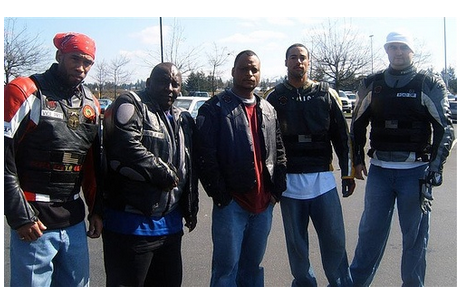
\includegraphics[width=\linewidth]{img/OriginalImage.png}
		\caption{Originalna slika}
	\end{subfigure}
	\begin{subfigure}[b]{0.4\linewidth}
		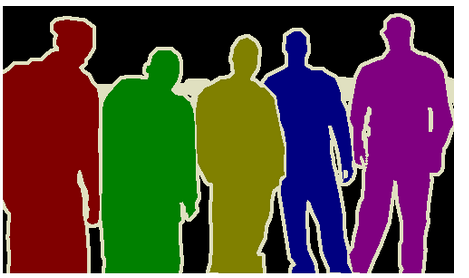
\includegraphics[width=\linewidth]{img/InstanceSegmentation.png}
		\caption{Instancijski segmentirana slika}
	\end{subfigure}
	\caption{Instancijska segmentacija slike, (Pascal VOC2007)}
	\label{img:instanceSegmentation}
\end{figure}

\bigskip
\item Ostale, manje zastupjene, kategorije računalnog vida : Super-resolution, Style Transfer, Colourisation 

\begin{figure}[htp]
	\centering
	\begin{subfigure}[b]{0.4\linewidth}
		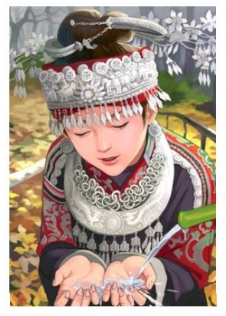
\includegraphics[width=\linewidth]{img/OriginalSRGAN.png}
		\caption{Originalna slika}
	\end{subfigure}
	\begin{subfigure}[b]{0.4\linewidth}
		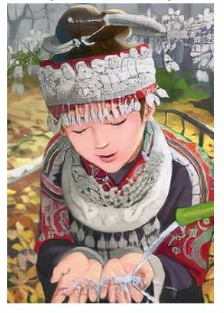
\includegraphics[width=\linewidth]{img/SRGAN.png}
		\caption{SRGAN}
	\end{subfigure}
	\caption{Slika poboljšana metodom Super-resolution GAN (Christian Ledig et al., 2016)}
	\label{img:SRGAN}
\end{figure}

\begin{figure}[htp]
	\centering
	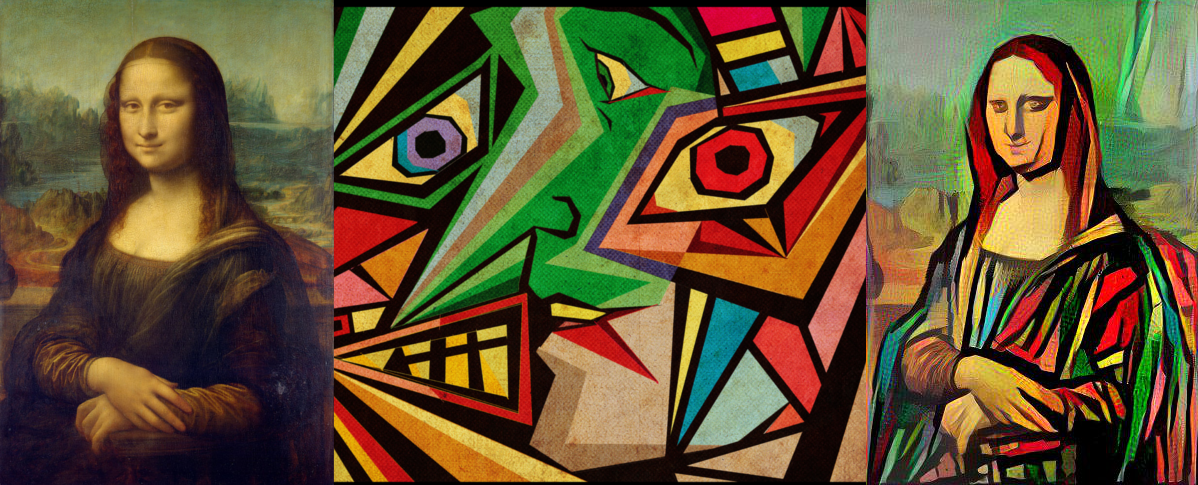
\includegraphics[width=\linewidth]{img/StyleTransfer.png}
	\caption{Prva slika prikazuje originalnu \textit{Mona Lisu}, druga slika prikazuje sliku naslikanu u stilu kubizma/ekspresionizma, treća slika prikazuje stil druge slike prenesen na prvu sliku}
	\label{img:styleTransfer}
\end{figure}

\begin{figure}[H]
	\centering
	\begin{subfigure}[b]{0.4\linewidth}
		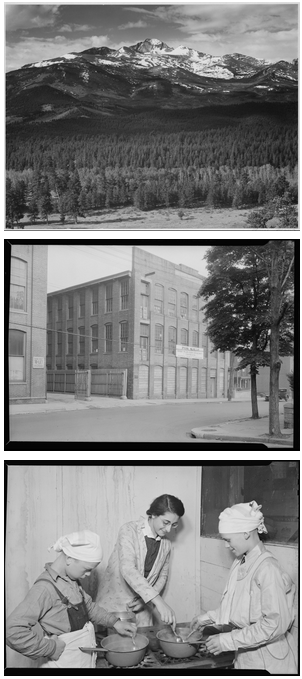
\includegraphics[width=\linewidth]{img/ColourisationOriginal.png}
		\caption{Originalna slika}
	\end{subfigure}
	\begin{subfigure}[b]{0.4\linewidth}
		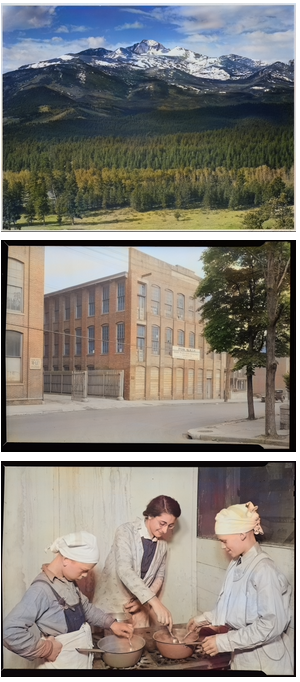
\includegraphics[width=\linewidth]{img/Colourisation.png}
		\caption{Colourisation}
	\end{subfigure}
	\caption{Slika poboljšana metodom colourisation}
	\label{img:colourisation}
\end{figure}

\end{enumerate}

U okviru ovoga rada pažnja je stavljena isključivo na \textbf{detekciju objekata}.

\chapter{Detekcija objekata prije konvolucijskih modela}
Povijest prepoznavanja (detekcije) objekata seže puno dalje od konvolucijskih neuronskih mreža. Prvi sustavi detekcije objekata problemu su prilazili geometrijski. Neki od takvih pristupa bili su:

\begin{itemize}
\item \textbf{poravnanje} gdje se pokušavalo pronaći takvu transformaciju slike koja bi minimizirala pogrešku:
\[\sum_{i} residual(T(x_i), x_i')\]

Ovaj period trajao je od ranih 60ih do početka 90ih godina prošlog stoljeća. Uglavnom se pokušavalo riješiti problem detekcije razlamanjem objekata na slici u manje komponente (\textit{engl. Block world}, L. G. Roberts Machine Perception of Three Dimensional Solids, 1963.).
\item \textbf{modeli temeljeni na izgledu} (\textit{engl. appearance - based models}) su modeli temeljeni na svojstvenim vrijednostima (Eigenfaces for Recognition, Turk and Pentland, 1991.) te histogramima boja (Swain and Ballard, IJCV 1991.)
\item \textbf{klizeći prozor} pristup koji se donekle i danas primjenjuje. Ovaj pristup smatra se početkom "modernog doba" računalnog vida, iako se klizeći prozor koristi u najjednostavnijijm mogućim oblicima. Ovaj period počinje ranih 90ih godina, a predvode ih Turk and Pentland svojim radom "Eigenfaces for Recognition" izdanim 1991. godine, a vrhunac se potiže 2001. godine objavljivanjem algoritma koji su razvili Viola i Jones.
\item \textbf{lokalne značajke} (\textit{engl. local features}) gdje su oblici predmeta koje je potrebno detektirati djelomično poznati (D. Lowe, 2004.). U tom periodu Google razvija i prvi pretraživač slika. 
\item \textbf{parts-and-shape modeli} koji koriste kombinaciju više vrsta značajki: ponovo razlamaju objekte na dijelove, relativne odnose između tih dijelova te samu prisutnost dijelova objekta (Weber, Welling and Perona, 2000.).
\item \textbf{bags-of-features modeli} uvode prepoznavanje tekstura. Klasični bag-of-features modeli imaju standardizirane korake (\textit{engl. pipeline}): 
\begin{enumerate}
\item Feature extraction
\item Learn "visual vocabulary"
\item Quantize features using visual vocabulary
\item Represent images by frequencies of “visual words”
\end{enumerate}
\end{itemize}
\section{Viola-Jones algoritam}

Prije velikog razvoja konvolucijskih neuronskih mreža, Paul Viola i Michael Jones su 2001. godine u svom radu \citep{ViolaJones} objavili svoj algoritam koji je tada bio prvi algoritam koji je omogućavao detekciju lica u stvarnom vremenu. Iako se može trenirati i na drugim domenama, algoritam je najpoznatiji po detekciji lica pa će na toj domeni ovdje biti i opisan.

Naravno, algoritam treba puno pozitivnih (slike lica) i negativnih primjera (slike bez lica). Iz tih slika potrebno je izvući značajke prema kojima će kasnije biti moguće odrediti (detektirati) lice. Za ekstraciju značajki koriste se Haarove značajke.

\begin{figure}[htb]
	\centering
	\begin{subfigure}[b]{0.4\linewidth}
		
\includegraphics[width=\linewidth]{img/EdgeFeatures.png}
		\caption{Značajke rubova}
		\label{img:haar-features1}
	\end{subfigure}
	\begin{subfigure}[b]{0.4\linewidth}
		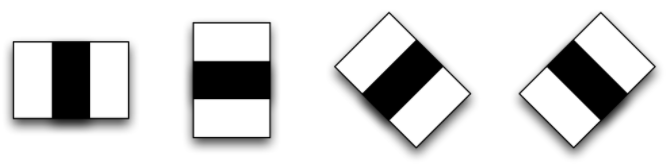
\includegraphics[width=\linewidth]{img/LineFeatures.png}
		\caption{Linijske značajke}
		\label{img:haar-features2}
	\end{subfigure}
	\begin{subfigure}[b]{0.4\linewidth}
		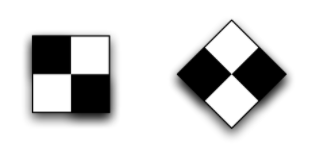
\includegraphics[width=\linewidth]{img/DiagonalFeatures.png}
		\caption{Dijagonalne značajke}
		\label{img:haar-features3}
	\end{subfigure}
	\begin{subfigure}[b]{0.4\linewidth}
		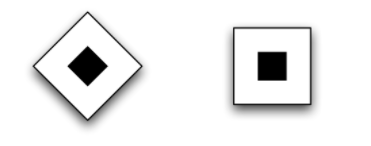
\includegraphics[width=\linewidth]{img/CenterSorround.png}
		\caption{Radijalne značajke}
		\label{img:haar-features4}
	\end{subfigure}
	\caption{Haarove značajke}
	\label{img:haar-features}
\end{figure}

Haarove značajke računaju se na temelju razlike u intenzitetu piksela. Primjerice, ako su vrijednosti piksela u rasponu od 0 (bijeli piksel) do 1 (crni piksel), svi pikseli koji imaju vrijednost veću do 0.5 smatraju se tamnim, a svi pikseli koji imaju vrijednost manju od 0.5 smatraju se svijetlima. Na slici \ref{img:haar-features} prikazane su 4 kategorije Haarovih značajki. Dakle, kako bi bilo moguće odrediti gdje se na slici nalazi (i ako se nalazi) neka od značajki, slika se dijeli na manja područja te se na svakom od tih područja traže Haarove značajke. Naravno, značajke se skaliraju i rotiraju kako bi se pronašli svi dijelovi slike koji zadovoljavaju uvjete značajki. Zatim se odredi gledano područje, kao što to prikazuje slika \ref{img:haar-calc}, te se računaju vrijednosti za Haarove značajke po formuli:
\[
\Delta = dark - white = \frac{1}{n}\sum_{}^{n}I_{dark}(x) - \frac{1}{n}\sum_{}^{n}I_{light}(x)
\]

\begin{figure}[htb]
	\centering
	\begin{subfigure}[b]{0.4\linewidth}
		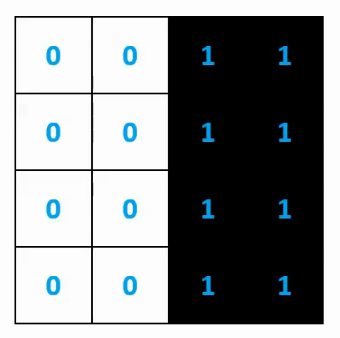
\includegraphics[width=\linewidth]{img/IdealHaarFeatures.png}
		\caption{Idealne vrijednosti piksela}
		\label{img:haar-ideal-features}
	\end{subfigure}
	\begin{subfigure}[b]{0.4\linewidth}
		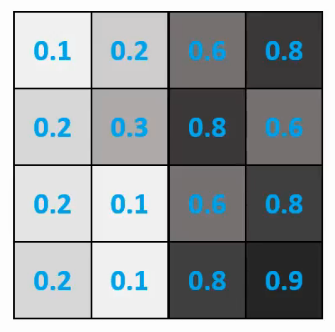
\includegraphics[width=\linewidth]{img/RealHaarFeatures.png}
		\caption{Stvarne vrijednosti piksela}
		\label{img:haar-real-features}
	\end{subfigure}
	\caption{Izračun za linijske Haarove značajke}
	\label{img:haar-calc}
\end{figure}


Slika \ref{img:haar-features1} prikazuje Haarove značajke rubova. Neke od primjena tih značajki su detekcija obrva, gornje/donje usne i zubi. Slika \ref{img:haar-features2} prikazuje linijske Haarove značajke koje služe za detekciju nosa, usta, očiju itd. Nadalje, slika \ref{img:haar-features3} prikazuje dijagonalne Haarove značajke koje se koriste u detekciji složenijih karakteristika. Recimo, ako se lice na slici smije, rubovi usana se uvuku u obraze te su tada slabije osvjetljeni. Tako zajedno sa okom na istoj strani lica tvore tamnije zone, dok obraz i nos čine svijetlija područja. Zadnja skupina Haarovih značajki su radijalne Haarove značajke koje prikazuje slika \ref{img:haar-features4}. Te se značajke koriste u detekciji zjenica, rubova usana i sl. Dakle, Haarove značajke mogu se shvatiti kao preteča konvolucijskih jezgri. Slika \ref{img:haar-image} prikazuje neke od haarovih značajki detektiranih na slici.

\begin{figure}[htb]
	\centering
	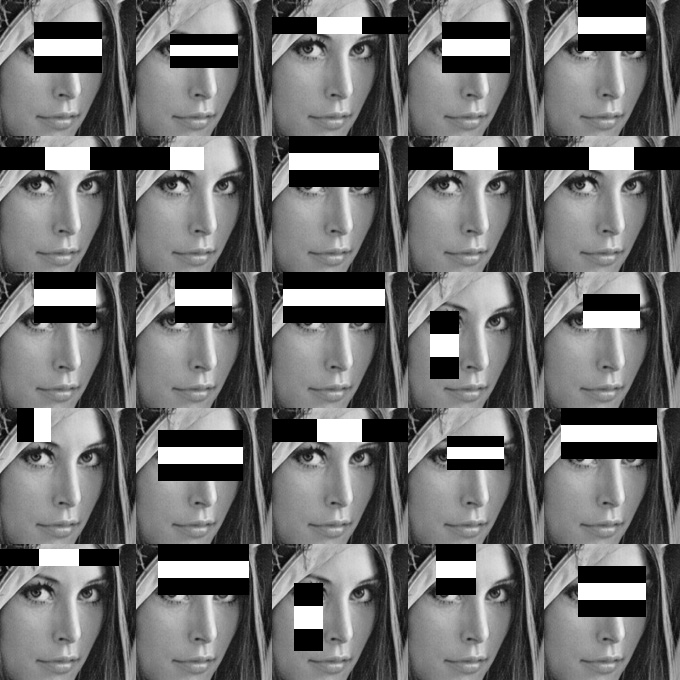
\includegraphics[width=12cm]{img/Haar3.jpg}
	\caption{Neke od Haarovih značajki pronađenih na slici}
	\label{img:haar-image}
\end{figure}

Ovaj proces je dosta spor i neefikasan jer se na ovakav način dođe do više od 160000 različitih značajki. Očito je da, ovisno o domeni, neke od značajki odgovaraju više od drugih, no javlja se pitanje kako odabrati najbolje značajke? Odgovor na ovo pitanje je Adaboost algoritam. Adaboost (skraćeno od \textit{engl. Adaptive Boosting}) je algoritam osmišljen 2003. godine koji kombinira izlaze iz ostalih, "slabijih" kalsifikatora, te njihovom težinskom sumom dolazi do optimuma algoritma. Adaboost zapravo uči i optimizira težine za svaki od klasifikatora.

\begin{figure}[htb]
	\centering
	
\includegraphics[width=\linewidth]{img/Viola-Jones.png}
	\caption{Viola-Jones algoritam}
	\label{img:viola-jones}
\end{figure}

Autori su došli do zaključka da je čak sa samo 200 značajki moguće postići točnost pronalaženja lica od 95\%. Konačne postavke algoritma iz rada \citep{ViolaJones} sadržavale su oko 6000 značajki. Kako bi optmimizirali ovaj složeni proces i izbjegli primjenu svih 6000 značajki na svaku sliku, Viola i Jones odlučili su napraviti strukturu kaskada značajki u kojoj svaka iduća razina ima sve složenije Haarove značajke. Kao što je označeno na slici \ref{img:haar-cascades}, svaka razina ima mogućnost odbaciti sliku ukoliko ne nađe značajke svoje razine na slici. Tako se dijelovi slike koji ne prikazuju lice odbacuju te se oslobađaju računalni resursi za procesiranje slika na kojima se nalazi lice. Autori navode da je prosjek značajki evaluiranih po slici oko 10.

\begin{figure}[htb]
	\centering
	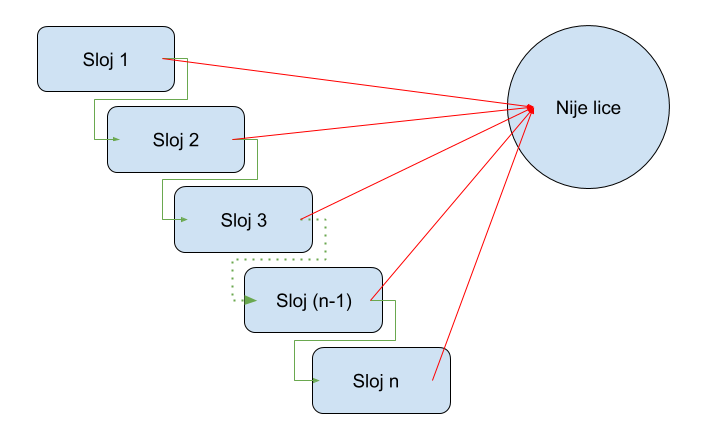
\includegraphics[width=\linewidth]{img/HaarCascades.png}
	\caption{Kaskada Haarovih značajki}
	\label{img:haar-cascades}
\end{figure}

\begin{figure}[htb]
	\centering
	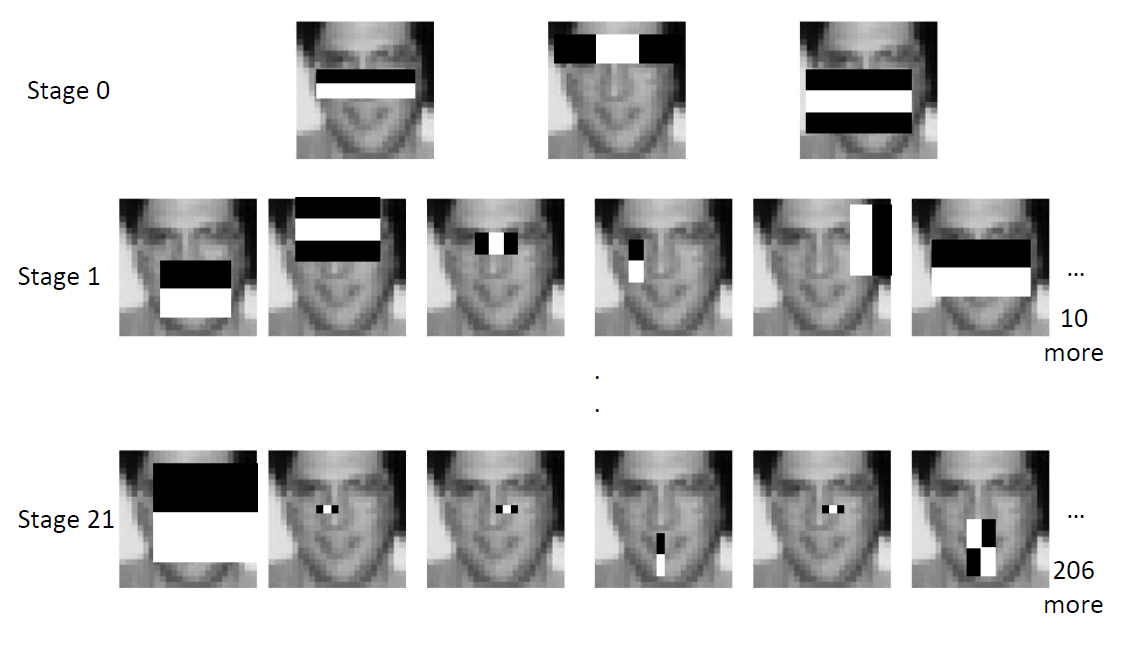
\includegraphics[width=\linewidth]{img/haar2.jpg}
	\caption{Dijelovi Haarovih značajki pronađeni na različitim razinama kaskada}
	\label{img:haar-cascade-layers}
\end{figure}

Rezultati ovih slabijih klasifikatora kombiniraju se u konačni klasifikator koji odlučuje nalazi li se lice na slici. 

Viola-Jones algoritam je svojedobno bio vrlo popularan algoritam jer nudi vrlo pouzdane rezultate, obradu u stvarnom vremenu i invarijantnost na skaliranje. No, isto tako, ima i nekoliko nedostataka kao što su netolerantnost na rotaciju, osjetljivost na osvjetljenje objekata na slici i sl. Činjenica da se još i danas koristi govori dovoljno o kvaliteti i važnosti ovog algoritma.


\chapter{Detekcija objekata konvolucijskim modelima}
\section{Neuronske mreže}

\subsection{Neuron}

Neuronske mreže nastale su kao rezultat pokušaja reprodukcije rada ljudskog mozga.

Osnovna gradivna jedinica ljudskog mozga jest neuron. Ljudski mozak sastavljen je od oko $10^11$ neurona kojih ima više od 100 vrsta i koji su shodno svojoj funkciji raspoređeni prema točno definiranom 
rasporedu. Svaki je neuron u prosjeku povezan s $10^4$ drugih neurona. Četiri su osnovna dijela neurona: tijelo stanice (soma), skup dendrita (ogranaka), aksona (dugačke cijevčice koje prenose električke poruke) i niza završnih članaka 

\begin{figure}[htb]
\centering
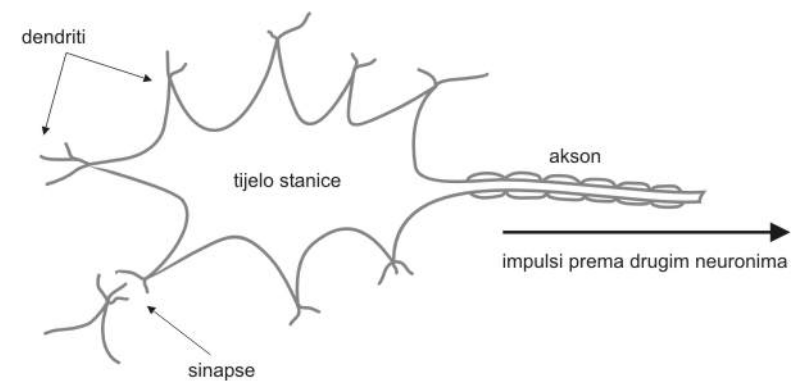
\includegraphics[width=8cm]{img/Neuron.png}
\caption{Građa neurona}
\label{img:human-neuron}
\end{figure}

Tijelo stanice sadrži informaciju predstavljenu električkim potencijalom između unutrašnjeg i vanjskog dijela stanice (oko –70 mV u neutralnom stanju). Na sinapsama, spojnom sredstvu dvaju neurona kojim su pokriveni dendriti, primaju se informacije od drugih neurona u vidu post-sinaptičkog potencijala koji utječe na potencijal stanice povećavajući (hiperpolarizacija) ili smanjivajući ga (depolarizacija). U tijelu stanice sumiraju se post-sinaptički potencijali tisuća susjednih neurona, u ovisnosti o vremenu dolaska ulaznih informacija. Ako ukupni napon pređe određeni prag, neuron "pali" i generira tzv. akcijski potencijal u trajanju od 1 ms. Kada se informacija akcijskim potencijalom prenese do završnih članaka, onda oni, ovisno o veličini potenijala, proizvode i otpuštaju kemikalije, tzv. neurotransmitere. To zatim ponovno inicira niz opisanih događaja u daljnjim neuronima. Propagacija impulsa očigledno je jednosmjerna. 

Funkcionalnost biološkog neurona imitira McCulloch-Pitts model umjetnog neurona, tzv. \textit{Threshold Logic Unit} (TLU). Model koristi slijedeću analogiju: signali su opisani numeričkim iznosom i na ulazu u neuron množe se težinskim faktorom koji opisuje jakost sinapse; signali pomnoženi težinskim faktorima zatim se sumiraju analogno sumiranju potencijala u tijelu stanice; ako je dobiveni iznos iznad definirana praga, neuron daje izlazni signal. 

U općenitom slučaju, umjetni neuron umjesto funkcije praga može imati i neku drugu funkciju, tzv. aktivacijsku funkciju (transfer funkcija, prijenosna funkcija). Općeniti model umjetnog neurona nalazi se na slici \ref{img:artificial-neuron}. U nastavku ćemo za pojam umjetni neuron ravnopravno koristiti i istovjetne pojmove: čvor ili jedinica. 

\begin{figure}[htb]
\centering
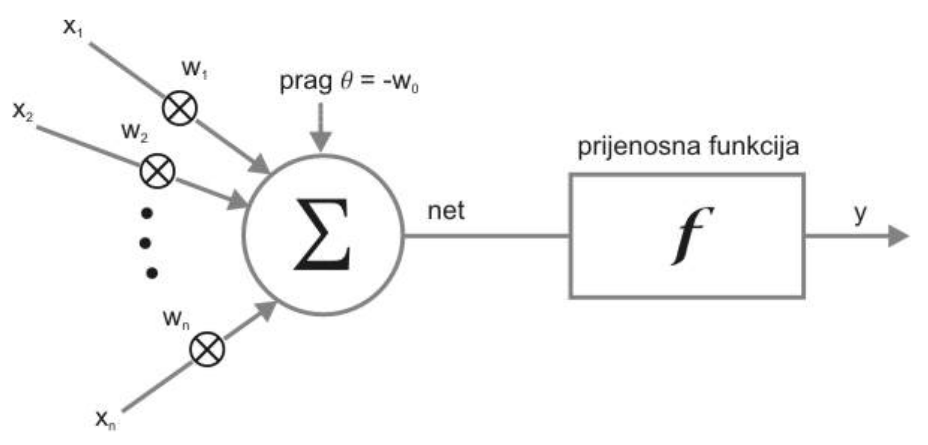
\includegraphics[width=8cm]{img/ArtificialNeuron.png}
\caption{Umjetni neuron}
\label{img:artificial-neuron}
\end{figure}

Ulazne signale (njih ukupno $n$) označavamo sa $x_1, x_2, x_3, ... , x_n$, a pripadajuće težine označavamo sa $\omega_1, \omega_2, \omega_3,..., \omega_n$.
Ulazni signali općenito su realni brojevi u intervalu $[-1,1]$, $[0,1]$ ili samo elementi iz $\{0,1\}$, kada govorimo o Booleovom ulazu. Težinska suma $net$ dana je formulom \ref{eq:weighted-sum}. Zbog kompaktnosti se često dogovorno uzima da je vrijednost praga $\theta = --\omega_0$ te se dodaje ulazni parametar $x_0$ s fiksiranom vrijednošću 1, te tada \ref{eq:weighted-sum} izgleda:

\begin{equation}
net = \omega_1 x_1 + \omega_2 x_2 + ... + \omega_n x_n - \theta
\label{eq:weighted-sum}
\end{equation}

\begin{equation}
net = \omega_0 x_0 + \omega_1 x_1 + \omega_2 x_2 + ... + \omega_n x_n = \sum_{i=0}^{n} \omega_i x_i
\label{eq:weighted-sum_2}
\end{equation}

Izlaz $y$ je rezultat aktivacijske funkcije te ga zapisujemo:

\begin{equation}
y = f(\sum_{i=0}^{n} \omega_i x_i) = f(net)
\label{eq:activation-function}
\end{equation}


\subsection{Svojstva umjetne neuronske mreže}

Umjetna neuronska mreža (\textit{engl.} Artificial Neural Network, ANN) u širem je smislu riječi umjetna replika ljudskog mozga kojom se nastoji simulirati postupak učenja. Nešto stroža definicija bila bi skup međusobno povezanih jednostavnih procesnih elemenata, \textit{jedinica} ili \textit{čvorova}, čija se funkcionalnost temelji na biološkom neuronu. Pri tome je obradbena moć mreže pohranjena u snazi veza između pojedinih neurona tj. težinama do kojih se dolazi postupkom prilagodbe odnosno učenjem iz skupa podataka za učenje. Neuronska mreža obrađuje podatke distribuiranim paralelnim radom svojih čvorova.

To je paradigma kojom su implementirani pojednostavljeni modeli što sačinjavaju biološku neuronsku mrežu. Ova je analogija vrlo poopćena jer, naravno, postoje još mnogi fenomeni živčanog sustava koji nisu modelirani ovim pristupom. Također, postoje i karakteristike umjetnih neuronskih mreža koje se ne poklapaju sa onima živčanog sustava.

Prednosti neuronskih mreža nad standardnim (simboličkim) načinom obrade podataka:

\begin{itemize}
\item Vrlo su dobre u procjeni nelineranih odnosa uzoraka
\item Mogu raditi s nejasnim ili manjkavim podacima tipičnim za podatke iz različitih senzora, poput kamera i mikrofona, i u njima raspoznavati uzorke
\item Robusne su na pogreške u podacima, za razliku od konvencionalnih metoda koje pretpostavljaju normalnu raspodjelu obilježja u ulaznim podacima
\item Stvaraju vlastite odnose između podataka koji nisu zadani na ekplicitan simbolički način
\item Mogu raditi s velikim brojem varijabli ili parametara
\item Prilagodljive su okolini
\item Moguća je jednostavna VLSI implementacija (\textit{engl.} Very-large-scale integration)
\item Sposobne su formirati znanje učeći iz iskustva (tj. primjera)
\end{itemize}

Neuronske mreže odlično rješavaju sve probleme kod kojih postoji odnos između prediktorskih (ulaznih) i zavisnih (izlaznih) varijabli, bez obriza na visoku složenost te veze (nelinearnost) -- \textit{klasifikacija} i \textit{regresija} (\textit{predviđanje}). Neuronske mreže uključuju se u sve više pordučja, a primjeri domena na kojima se već široko primjenjuju su:

\begin{itemize}
\item raspoznavanje uzoraka
\item obrada slike
\item obrada teksta
\item obrada govora (zvuka)
\item problemi optimizacije
\item nelinearno upravljanje
\item obrada nepreciznih i nekompletnih podataka
\item simulacije i mnogi drugi
\end{itemize}


\subsection{Aktivacijske funkcije}

\subsubsection{Adaline}

Adaline (\textit{engl. Adaptive Linear Element}) aktivacijska funkcija je prva aktivacijska funkcija ikada te dijeli ime sa neuronom koji ju koristi. Zbog svojeg ranog razvoja, naravno da je i najjednostavnija:

\begin{equation}
f(net) = net
\label{eq:Adaline aktivacijska funkcija}
\end{equation}

Izlaz iz takve jedinice upravo je težinska suma njegovih ulaza. Dakle, izlaz odgovara općenitom modelu umjetnog neurona prikazanom na slici \ref{img:artificial-neuron}, a dan je izrazom \ref{eq:activation-function}.

\subsubsection{Funkcija skoka}

Funkcija skoka ili praga (\textit{engl. Threshold Logic Unit, TLU}) na izlazu daje Booleov izlaz ($\{False, True\}, \{0, 1\}$). Graf TLU dan je slikom \ref{img:tlu}.

\begin{equation}
f(net)=\left\{
\begin{array}{c l}	
     0 & $\textit{za net} $ < $ $ 0,\\
     1 & $\textit{inače}$
\end{array}\right.
\label{eq:Funkcija skoka}
\end{equation}

\begin{figure}[H]
\centering
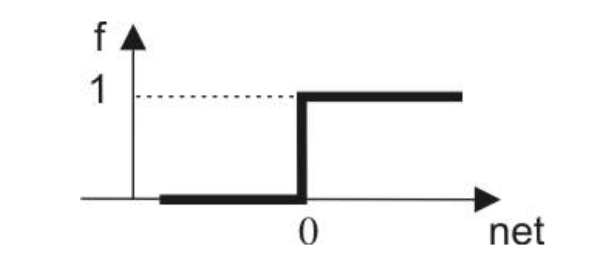
\includegraphics[width=8cm]{img/TLU.png}
\caption{Funkcija skoka}
\label{img:tlu}
\end{figure}

Znak nejednakosti u funkciji skoka, dodatno može u nekim slučajevima sadržavati i znak jednakosti čime se funkcija \ref{eq:tlu} mijenja u \ref{eq:linear-tlu}

\begin{equation}
f(net)=\left\{
\begin{array}{c l}	
     0   & $\textit{za net} $ \leq $ $ a,\\
     net & $\textit{za a} $ < $ \textit{net} $ < $ $ b,\\
     1   & $\textit{za net} $ \geq $ $ b
\end{array}\right.
\label{eq:Funkcija skoka koja je na dijelovima linearna}
\end{equation}

\begin{figure}[H]
\centering
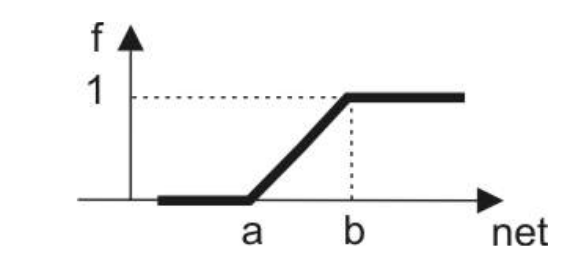
\includegraphics[width=8cm]{img/LinearTLU.png}
\caption{Na dijelovima linearna TLU}
\label{img:linear-tlu}
\end{figure}

Najčešća aktivacijska funkcija jest sigmoida. Vrlo važno svojstvo ove funkcije koje ju razlikuje od dosad navedenih funkcija jest da je derivabilna. To će se pokazati kao vrlo važna značajka za proces učenja neuronske mreže. Sigmoida je definirana kao:

\begin{equation}
f(net) = \frac{1}{1 + e^{-a net}}
\label{eq:sigmoid}
\end{equation}

\begin{figure}[H]
\centering
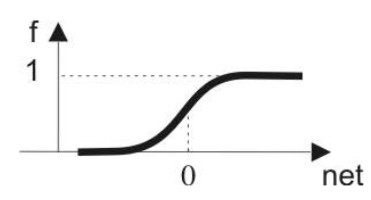
\includegraphics[width=8cm]{img/Sigmoid.png}
\caption{Sigmoidlana (logistička) funkcija}
\label{img:sigmoid}
\end{figure}

gdje parametar $a$ određuje nagib funkcije. Vrlo važno svojstvo sigmoide je da sve brojeve iz bilo kojeg intervala preslikava na raspon $[0,1]$. Zbog toga vrlo često izlaz iz logističke funkcije ima vjerojatnosnu interpretaciju, odnosno koristi se kada je na izlazu potrbno predvijeti vjerojatnosti. Važno je napomenuti da se sigmoida u području strojnog učenja koristi kada model ima binarni izlaz (predviđa 2 klase), dok se za višeklasnu regresiju/klasifikaciju koristi softmax:

\begin{equation}
f(net) = \frac{e^{net_i}}{\sum_{j=1}^{k} e^{net_j}}
\label{eq:sigmoid}
\end{equation}

\begin{figure}[H]
\centering
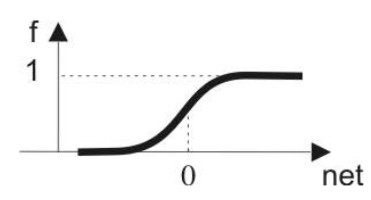
\includegraphics[width=8cm]{img/Sigmoid.png}
\caption{Sigmoidlana (logistička) funkcija}
\label{img:sigmoid}
\end{figure}

Softmax je generalizirana sigmoida. Izlaz iz funkcije softmax također vrlo često ima vjerojatnosnu interpretaciju. 

Zadnja aktivacijska funkcija koju ovdje valja spomenuti je ReLU (\textit{engl. Rectified Linear Unit}). 

\begin{equation}
f(net) = max(0, net)
\label{eq:relu}
\end{equation}

\begin{figure}[H]
\centering
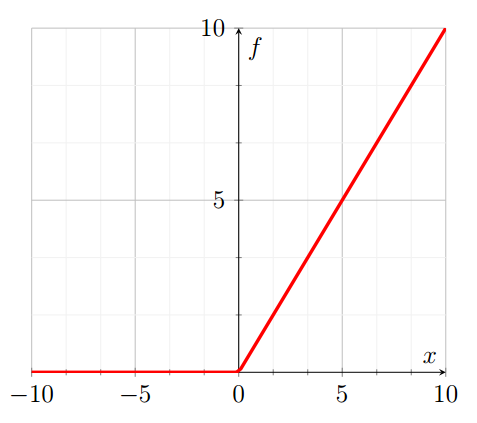
\includegraphics[width=8cm]{img/ReLU.png}
\caption{ReLU}
\label{img:relu}
\end{figure}

Ova aktivacijska funkcija je vrlo raširena u računalnom vidu i vrlo popularna kod konvolucijskih neuronskih mreža. Problem je što ova funkcija sve negativne vrijednosti stavlja u $0$ što smanjuje mogućmost modela da potpuno izvuče znanje iz podataka. Zato je osmišljena još jedna funkcija koja ne preslikava negativne vrijednosti u 0, nego u neku vrijednost blizu $0$ (što je vrijednost negativnija, preslikava se u vrijednost dalje od $0$). Ta funkcija naziva se "Leaky ReLU":

\begin{equation}
f(net)=\left\{
\begin{array}{c l}	
     a {net}   & $\textit{za net} $ < $ $ 0,\\
     {net}     & $\textit{za net} $ \geq $ $ 0
\end{array}\right.
\label{eq:Leaky ReLU}
\end{equation}

\begin{figure}[H]
\centering
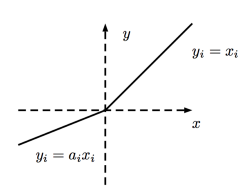
\includegraphics[width=8cm]{img/LeakyReLU.png}
\caption{Leaky ReLU}
\label{img:Leaky ReLU}
\end{figure}



sources: https://medium.com/the-theory-of-everything/understanding-activation-functions-in-neural-networks-9491262884e0
\section{Konvolucijske neuronske mreže}

Konvolucijske neuronske mreže mogu se zamisliti kao svojevrsno proširenje klasičnih višeslojnih neuronskih mreža. 

\chapter{Skupovi podataka}

\chapter{Opis alata}

\chapter{Implementacija}

\chapter{Zaključak}
Zaključak.

\bibliography{literatura}
\bibliographystyle{fer}

\begin{sazetak}
Sažetak na hrvatskom jeziku.

\kljucnerijeci{Ključne riječi, odvojene zarezima.}
\end{sazetak}

% TODO: Navedite naslov na engleskom jeziku.
\engtitle{Title}
\begin{abstract}
Abstract.

\keywords{Keywords.}
\end{abstract}

\end{document}
